\chapter{Methodology}
\label{c:methodology}

In this chapter, we describe the FileFarm system in detail. It starts by presenting the system architecture and roles in the system. Then it shows the model of each building block of FileFarm and the upload / download process flows. Finally it explains each of the desired characteristics FileFarm provides and the mechanisms behind them.

% system architecture
\section{System Architecture}
\label{s:systemarchitecture}

\begin{figure}[hbt]
\centering
  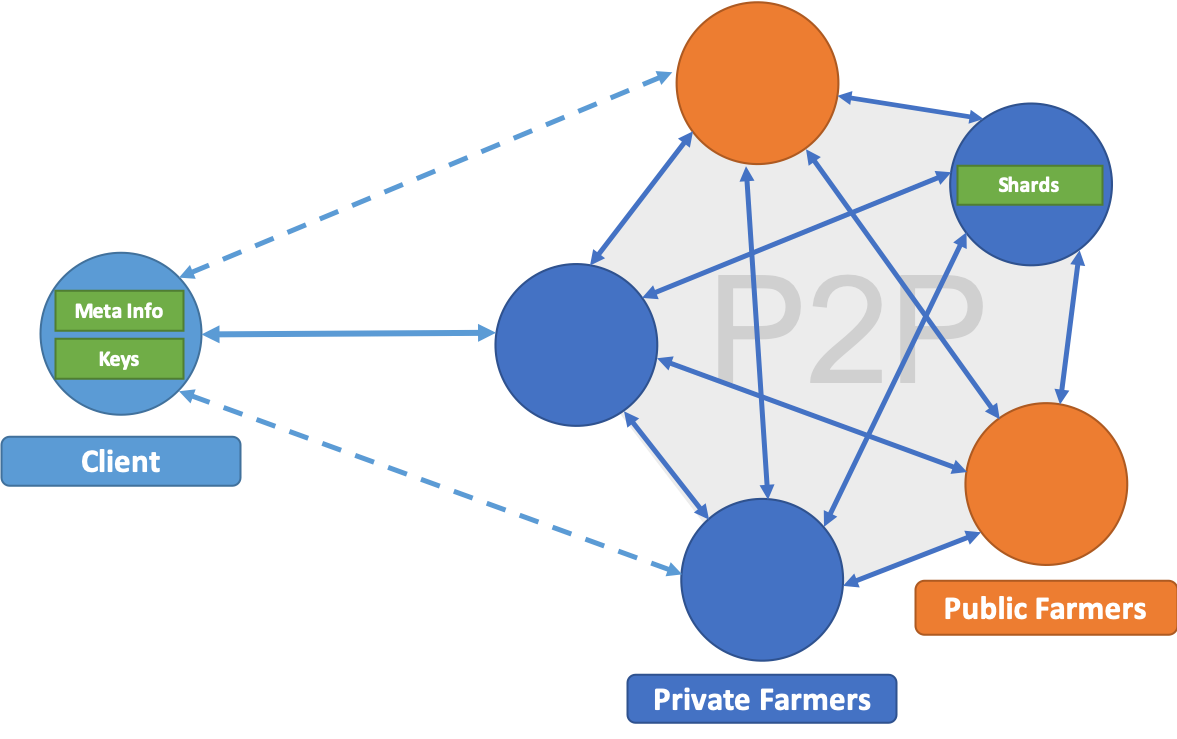
\includegraphics[width=15cm]{figures/system_architecture.png}
  \caption{System architecture}
  \label{fig:systemarchitecture}
\end{figure}

\newpage

The FileFarm system is composed of 2 roles:

\begin{enumerate}
  \item $Client$: User-side application providing user interface, handling upload/download tasks and managing file meta along with hash values and encryption keys for later retrieval.
  \item $Farmer$: Basic component of the FileFarm storage network. A farmer is linked with exactly 1 storage provider (either a public cloud or a private data server) to offer storage service. At the same time, farmers connect to each other to form a P2P network and take care of availability of each stored piece of data. A farmer also provides API for clients to store and retrieve data.
\end{enumerate}

As shown in Figure \ref{fig:systemarchitecture}, The FileFarm cloud-of-clouds is formed by farmers, in a sense that service availability has no dependence on any single farmer or its underlying cloud. Thus, FileFarm system has no single-point-of-failure. All farmers provide the same storage service. Thus, client can establish stateless connection with any farmer for uploading/downloading data.

The basic unit of data in FileFarm network is called $shard$, which is a computed segmentation of file that is saved in the network. A specific amount of distinct shards are required to reconstruct the original file, depending on the $sharding$ $schema$. From client's point of view, a file is split, encrypted and then computed into a number of shards with IDA (more details explained in \ref{s:dataconfidentiality}). Instead of the original file, the shards are what actually uploaded. The encryption keys, hashes, file meta are kept by client itself. This ensures that only the client itself is able to reconstruct its own data.

\newpage

% application models and process flows
\section{Application Models and Process Flows}
\label{s:applicationmodelsandprocessflows}

\begin{figure}[hbt]
\centering
  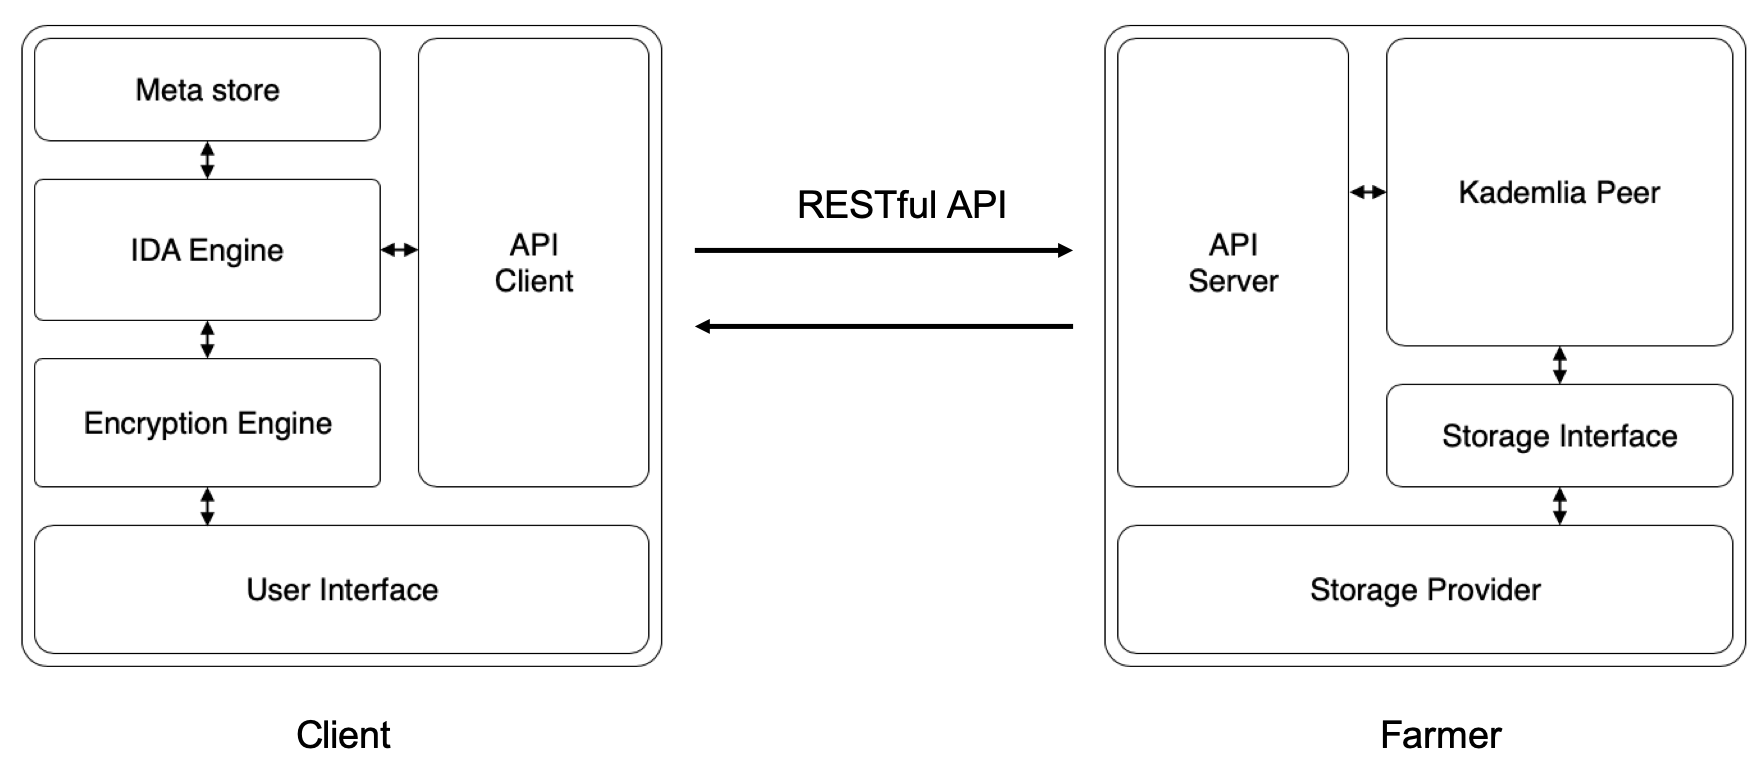
\includegraphics[width=14cm]{figures/application_models.png}
  \caption{Application model of client and farmer}
  \label{fig:applicationmodels}
\end{figure}

Figure \ref{fig:applicationmodels} shows the model of client and farmer applications. Client application has a interface for user to manage their own storage and to upload/download files. When receiving command from user to upload a file, the client application splits the file into slices and pre-process each slice with encryption engine and IDA engine. After pre-process, each slice is transformed into multiple shards, and the encryption keys and hash value of shards are saved in the client's meta store at the same time. The client application then upload each shard to the FileFarm storage network through a randomly-chosen farmer. Farmer application, on the other hand, has a API server module that serves request from client applications. Besides the server module, farmer also has a Kademlia peer module that coordinates with other farmer's corresponding part to synchronize storage status of uploaded shards and provide an efficient way to locate them. In order to apply farmer application on different storage services, FileFarm implements an abstract storage interface layer that provides identical out-bounded API but negotiate with different storage providers according to their API format.

Going with the application model, we present upload / download flow of FileFarm in figure \ref{fig:uploadflow} and figure \ref{fig:downloadflow}, respectively. Some of the processes in these 2 flow diagrams is not clear yet, which will be explained in the following sections.

\newpage

\begin{figure}[hbt]
\centering
  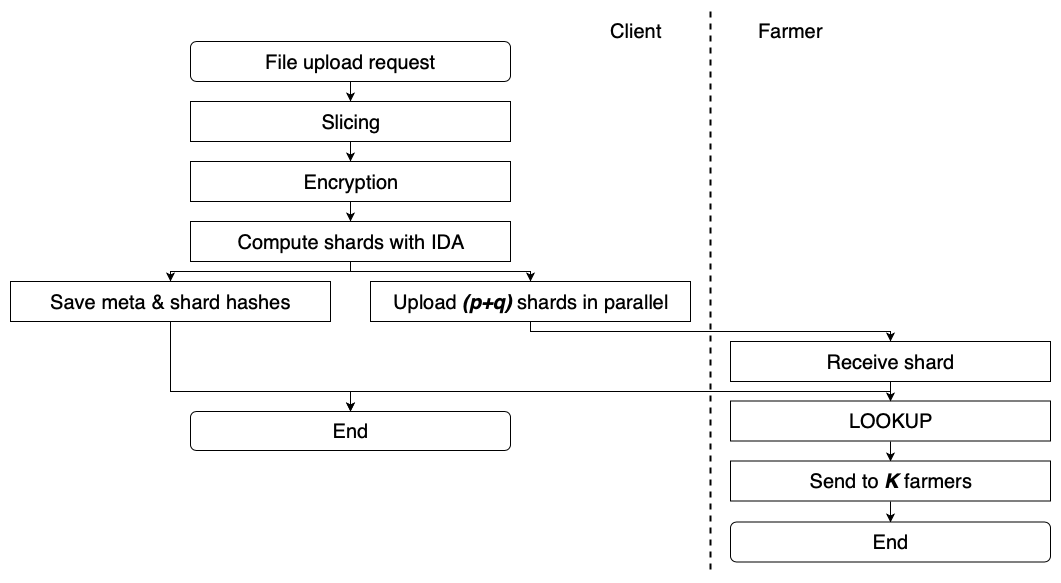
\includegraphics[width=11.5cm]{figures/upload_flow.png}
  \caption{Upload flow}
  \label{fig:uploadflow}
\end{figure}

\begin{figure}[hbt]
\centering
  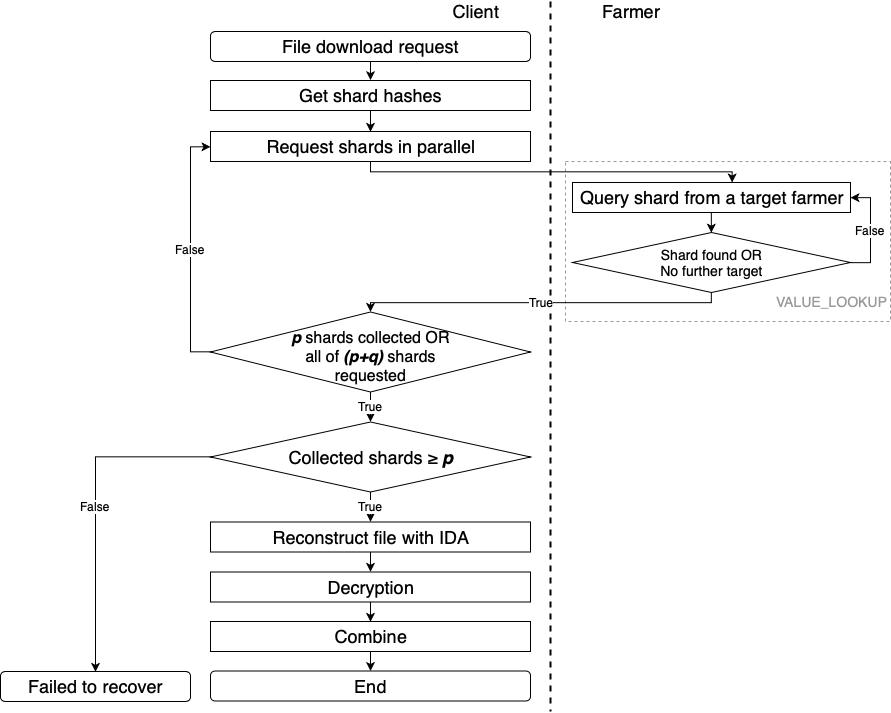
\includegraphics[width=14cm]{figures/download_flow.png}
  \caption{Download flow}
  \label{fig:downloadflow}
\end{figure}

\newpage

% DHT-based approach
\section{DHT-Based Approach}
\label{s:dhtbasedapproach}

To find shards in a P2P network, FileFarm implements Kademlia DHT protocol. Instead of saving location of shards as static records in a centralized database, FileFarm adopts Kademlia's dynamical look up procedures, as described in \ref{s:kademlia}. Before storing a shard, a farmer uses the LOOKUP procedure to determine on which farmers the shard should be stored, and then send parallel STORE RPCs to these farmers. In the case of shard retrieval (download), a farmer performs VALUE\_LOOKUP procedure to get find the shard iteratively until it is found. Both LOOKUP and VALUE\_LOOKUP procedures are robust to churn of farmers, network topology changes and even scale of network size, which usually can not be handled well in centralized solutions.

Kademlia protocol makes sure that:

\begin{enumerate}
  \item Each shard is stored on at least $K$ farmers, where $K$ is a configurable redundancy parameter
  \item It takes no more than $\lceil log(n) \rceil + c$ steps to find these $K$ farmers using LOOKUP procedure, where $n$ denotes network size.
  \item Shards are dispersed across entire network due to the randomly-assigned IDs, which balances farmers' load in terms of consumed storage size and request frequency.
\end{enumerate}

This gives FileFarm guarantees on $redundancy$, certain level of $I/O$ $efficiency$ and $load$-$balancing$. Besides, since given shard, the $K$ farmers to store it are uniquely defined and the results of LOOKUP and VALUE\_LOOKUP procedures have no dependence on originating node, a client can request any farmer to upload or download the shard, which will eventually be stored on the same set of farmers. This allows some favored service designs:

\begin{enumerate}
  \item A $fault$-$tolerant$ design in which clients do not rely on a specific farmer to perform upload / download tasks
  \item A $load$-$balancing$ design in which clients randomly choose farmers to perform upload / download tasks
  \item A $parallel$ design in which clients upload /download different shards from different farmers simultaneously
\end{enumerate}

\newpage

% Beyond DHT
\section{Beyond DHT}
\label{s:beyonddht}

From \ref{s:dhtbasedapproach}, we acknowledged that FileFarm inherits a number of performance benefits from Kademlia. However, these are not enough for a storage system, as DHTs are originally invented and applied to content-sharing applications but not storage systems. To serve as an enterprise storage, further requirements are taken into consideration:

\begin{enumerate}
  \item $Data$ $confidentiality$
  \item $Access$ $management$
  \item $Cost$ $efficiency$
  \item $Retrievability$
\end{enumerate}

\noindent To meet these requirements, we design corresponding mechanisms:

\begin{enumerate}
  \item $Encryption$ and $information$ $dispersal$ $algorithm$
  \item $Certificate$-$based$ $authentication$
  \item $Storage$ $release$ and $prioritized$ $download$
  \item $Public$ $farmer$ $ID$ $assignment$
\end{enumerate}

\noindent These requirements and their corresponding mechanisms will be explained in \ref{s:dataconfidentiality}, \ref{s:accessmanagement}, \ref{s:costefficiency}, \ref{s:retrievability}, respectively.

\begin{figure}[hbt]
\centering
  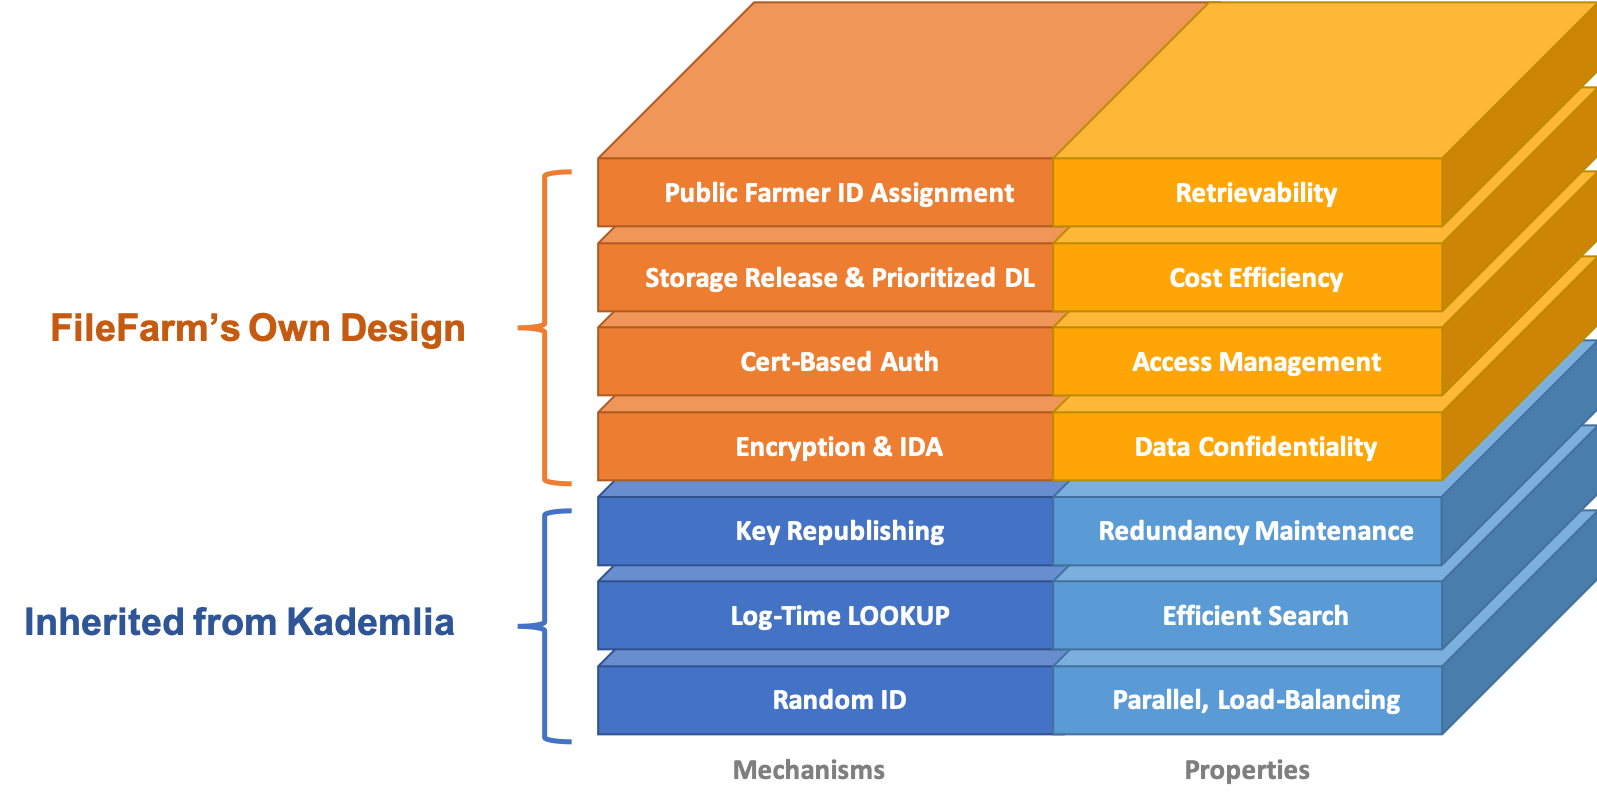
\includegraphics[width=14cm]{figures/property_stack.png}
  \caption{FileFarm's property stack}
  \label{fig:propertystack}
\end{figure}

% data confidentiality
\section{Data Confidentiality}
\label{s:dataconfidentiality}

In order to preserve privacy and confidentiality while storing data on public clouds, FileFarm introduces a pre-processing flow of files before they are actually uploaded, in a sense that every files are randomly dispersed over clouds, and only the owner holds the key to retrieving and reconstructing them. To be precise, an example is shown in Figure \ref{fig:dataconfidentiality}. A file $F$ of size $S$ is sliced into chunks $C1, C2, ..., Cn$ of size $\frac{S}{n}$ and then chunks are encrypted into $E1, E2, ..., En$ of the same size, respectively. For each of the encrypted chunk, a $sharding$ process is performed based on an Information Dispersal Algorithm of $(p,q)$ schema (see \ref{s:informationdispersalalgorithm}), which produces $(p+q)$ shards of size $\frac{S}{n}*\frac{p+q}{p}$, and the original encrypted chunk can be recovered from any $p$ of these $p+q$ shards. Now the pre-processing flow is finished, and the $n*(p+q)$ generated shards are uploaded to FileFarm in parallel.

To reconstruct the original file $F$, the procedure seems inverted. For each of the encrypted chunks $E1, E2, ..., En$ that was sharded into $p+q$ shards, the client sends parallel requests to collect $p$ shards so that it can be reconstructed by IDA. The reconstructed chunks are then decrypted to $C1, C2, ..., Cn$ and combined into the original file, $F$.

\begin{figure}[hbt]
\centering
  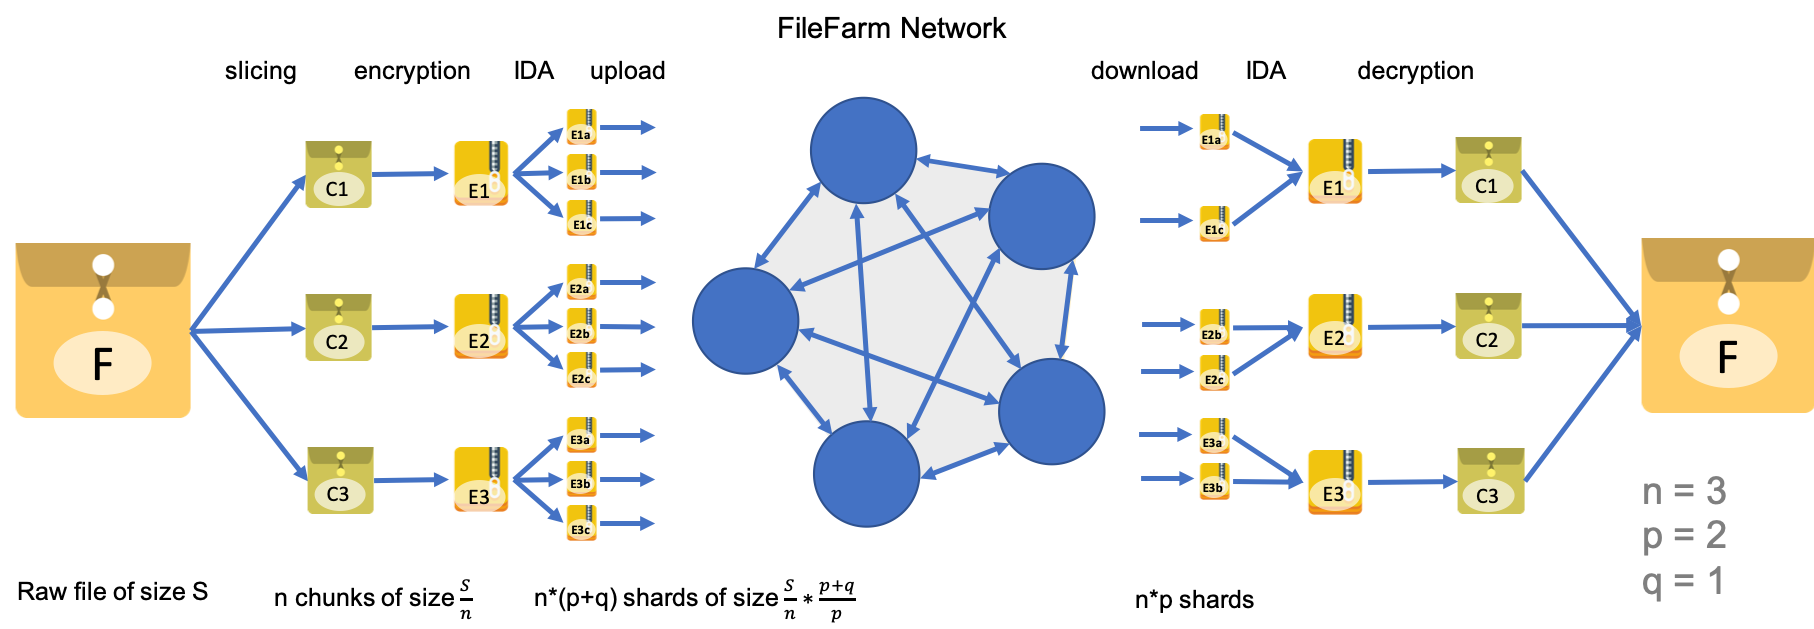
\includegraphics[width=15cm]{figures/data_confidentiality.png}
  \caption{An example of encryption and sharding flow}
  \label{fig:dataconfidentiality}
\end{figure}

\newpage

% access management
\section{Access Management}
\label{s:accessmanagement}

FileFarm aims to become an enterprise storage system applied in a private context. In such usage scenario, how to grant access to authorized clients while denying connections from unauthorized ones plays a crucial role in security of the system. To achieve this goal, FileFarm adopts a certificate-based approach toward access management.

\subsection{Certificate-Based Authentication}
\label{ss:certificatebasedauthentication}

\begin{figure}[hbt]
\centering
  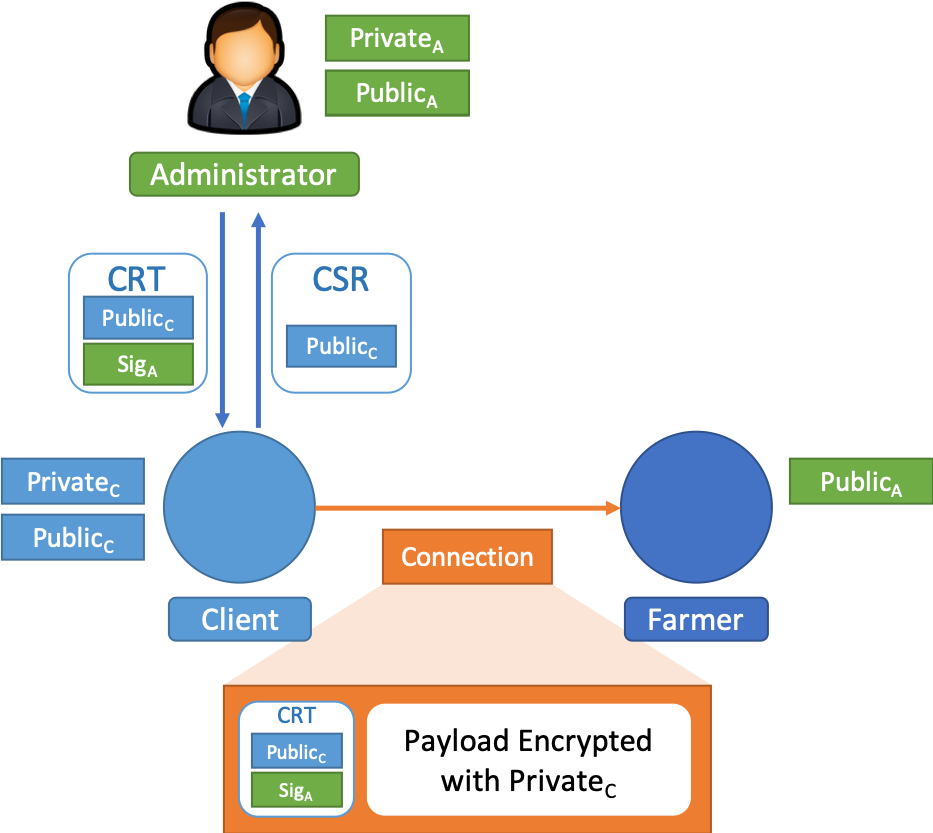
\includegraphics[width=14cm]{figures/access_management.png}
  \caption{An illustration of certificate-based authentication}
  \label{fig:accessmanagement}
\end{figure}

\newpage

This approach is based on the concept of Public Key Infrastructure, which is described in \ref{s:publickeyinfrastructure}, whereas the goal here is to validate clients but not serving hosts. The approach involves 3 kinds of roles: farmers, clients, and the administrator. When the administrator initializes the system, it generates a private/public key pair and install the public key on all launched farmers. When a client wants to access the FileFarm system, it generates a private/public key pair and sends a certificate signing request to the administrator, which includes the client's information along with its public key. On receiving such request, the administrator makes a decision on whether to grant access for the client or not. If the client passes administrator's validation, the administrator creates a signature on the signing request, which turns into a certificate. The certificate is then sent back to the client. With a certificate issued by the administrator, the client is now allowed to access the FileFarm storage network. To access FileFarm, the client appends its certificate to the connection request packet, and then encrypts the payload with its own private key. When receiving request from clients, a farmer check the validity of the certificate by verifying the signature on it using administrator's public key. The farmer also verifies client's identity by decrypting the payload using client's public key specified in the certificate.

\newpage

% cost efficiency
\section{Cost Efficiency}
\label{s:costefficiency}

To minimize the fee charged by storage provider without lost of retrievability, FileFarm implements 2 mechanisms that addresses different kind of charges, respectively.

\subsection{Storage Release}
\label{ss:storagerelease}

The storage release mechanism reduces "static storage fee" by releasing unused redundant shards. To understand how it works, we need to take a closer look at how the underlying Kademlia DHT protocol maintains redundancy. Kademlia implements an \textit{Efficient Key Republishing} mechanism that regularly checks if each shard is stored on the $K$ closest farmers.\cite{maymounkov2002kademlia} If any of the $K$ closest farmers does not store the shard, a copy will automatically be sent to it. This assurance is provided by the design in which each farmer periodically attempts to "republish" each shards it stored to the other $K-1$ farmers who should store the same shard. During the republishing period, if a farmer receives the republishing message of a shard from other farmer, it assumes the message has also been sent to the other $K-1$ closest farmers and thus it should not republish it again during this period in order to reduce traffic. As long as the republishing interval of farmers are not exactly matched, there will only be exactly 1 republishing message for each shard in each interval.

The efficient key republishing mechanism ensures that each shard will always have "at least" $K$ copies over the storage network. However, there are some scenarios that makes number of copies more than $K$, which results in unneeded storage overhead. The storage release mechanism is designed to eliminate this overhead. Considering a scenario in which a shard is kept by $K$ farmers and one of them churns off accidentally. With efficient key republishing, one of the remaining $K-1$
farmers will detect this and send a copy of the shard to the $K+1^{th}$ closest farmer, so that redundancy recovers from $K-1$ to $K$. However, when the failed farmer recovers from service outage, the redundancy will raise from $K$ to $K+1$. This is the moment that storage release mechanism should work. Due to the fact that republishing message will only be sent to the $K$ closest farmers, the $K+1^{th}$ closest farmer will not receive this message, which triggers it to republish the shard in the next period. To find the $K$ closest farmers to this shard, a LOOKUP procedure should be performed before sending republishing messages. This gives the $K+1^{th}$ closest farmer a chance to find itself not being one of the K closest farmers, it then stops the republishing process and deletes the shard from its storage. This shows the entire working procedure for storage release mechanism.

\subsection{Prioritized Download}
\label{ss:prioritizeddownload}

Prioritized download is a mechanism aiming to minimize "data transfer out" fee from public clouds. This mechanism only makes sense when applied in hybrid cloud settings, where not only public clouds but also enterprise's private storage machines such as NAS or SAN are contributed to the storage system. In hybrid-cloud settings, enterprises optionally build their own private farmers. The private farmers are usually not as reliable as public ones. However, they have advantages in at least 2 aspects:

\begin{enumerate}
  \item High throughput and low delay in local area network (LAN)
  \item No data transfer fee needed
\end{enumerate}

These advantages make it reasonable for enterprises to split a little portion of budgets on investment of private storage devices.

Within hybrid-cloud settings, prioritized download ensures that shards are preferred to be downloaded from private farmers. This not only reduces data transfer fee charged by public clouds, but also improves download performance, based on the advantages of private farmers listed above.

To understand how prioritized download works, we need to take a closer look at how the underlying Kademlia DHT protocol retrieves a shard. Kademlia implements an iterative VALUE\_LOOKUP procedure to retrieve shards. To be more specific, a farmer initializes a VALUE\_LOOKUP for a target $key$ by loading the $K$ closest farmers it already knows into a lookup table. For each of the farmers in the lookup table, it sends out a "FIND\_VALUE" message. If the recipient does store the shard, it will response with the shard directly; otherwise, it will response with the $K$ farmers it knows closest to the target $key$. In the former case, the VALUE\_LOOKUP procedure finishes since the shard has successfully been retrieved by the requesting farmer; in the latter case, the requesting farmer updates its lookup table with the returned $K$ farmers and then sends another "FIND\_VALUE" message to the closest farmer known so far that hasn't been queried. The procedure is repeated until the shard is found or all farmers in the lookup table have been queried, which is the failed case of retrieval.

\newpage

Prioritized download is a modified version of VALUE\_LOOKUP, with some noticeable differences:

\begin{enumerate}
  \item Prioritized download finishes once the target shard is found on a $private$ farmer.
  \item Prioritized download memorizes a public farmer who has the shard when finding such one, but not download from it immediately.
  \item Prioritized download downloads from a public farmer only if there is no private farmer found storing the target shard
\end{enumerate}

From the description above, we know that FileFarm treats public farmers and private farmers differently. In fact, a special approach is implemented by FileFarm to achieve this kind of differentiation. We will explain the details and the benefits brought by such differentiation in \ref{ss:publicfarmeridassignment}.

% retrievability
\section{Retrievability}
\label{s:retrievability}

In FileFarm's design, redundancy introduced by the $K$ factor of Kademlia and the $q$ factor of information dispersal algorithm both contribute to retrievability of files. However, to provide a more rigorous guarantee on retrievability in hybrid-cloud settings where reliability of public clouds and private servers differs greatly, we have to make sure every shards are saved on at least 1 public cloud with high probability. This demand gives rise to the design of $public$ $farmer$ $ID$ $assignment$.

\subsection{Public Farmer ID Assignment}
\label{ss:publicfarmeridassignment}

To differentiate public farmers from private ones, FileFarm gives public farmers a special identity. In the 160-bit farmer ID space, each public farmer is assigned with an ID with last 144 bits be '0', hence there can be at most $2^{16}=65536$ public farmers in the network. In contrast, ID of private farmers are generated randomly but cannot have last 144 bits be '0'. Besides, public farmer IDs are issued in bit-reversal permutation ordering. To be clear, we explain this kind of ordering in a simplified case where public IDs vary in the first 4 bits and have last 156 bits be '0' (see figure \ref{fig:bitreversalpermutationordering}). To generate ID for the $i^{th}$ public farmer, we reverse the binary representation of the number $i-1$ and assign the resulting binary string as the first 4 bits of the newly-generated ID. Following this rule, the first 4 bits of generated public IDs will be '0000', '1000', '0100', '1100', ...

With public farmer IDs being assigned in bit-reversal permutation ordering, we can be certain that public farmers are dispersed over the 160-bit ID space. Since that hash value of shards follow a uniform distribution over the 160-bit key space and that shards are stored on farmers with ID closest to its hash value, the dispersion of public farmer IDs makes them load-balanced in terms of storage usage and request frequencies. Besides, this explicit assignment also avoids the situation that public farmer's IDs distribute uneven over the network, which would cause disparity between retrievability of shards.

To sum up, the assigning rules of public farmer IDs bring following benefits:

\begin{enumerate}
  \item Provide an explicit rule to distinguish public farmers from private ones, which is needed for prioritized download (\ref{ss:prioritizeddownload}) to work
  \item Pose a strong guarantee on load-balancing of public farmers, which in further minimizes the reliance on any single public cloud
  \item Maximize the likelihood of each shard to be stored by at least one public farmer, which improves the average retrievability of each shard and thus enhances the overall retrievability of files
\end{enumerate}

\begin{figure}[hbt]
\centering
  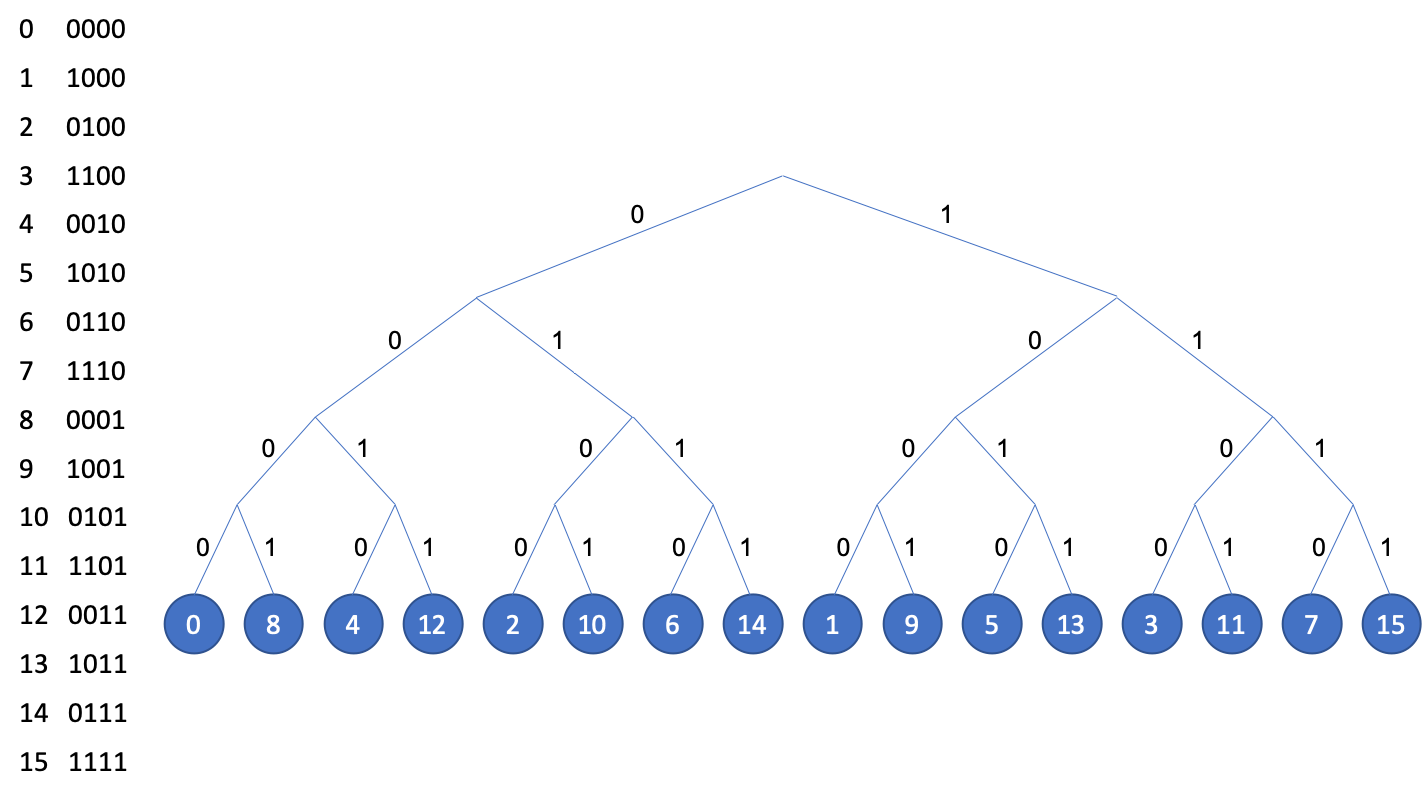
\includegraphics[width=16cm]{figures/bit_reversal_permutation_ordering.png}
  \caption{Bit-reversal permutation ordering with prefix length = 4}
  \label{fig:bitreversalpermutationordering}
\end{figure}